\section{Os pensadores e a origem da Geologia}
\subsection{Nicolas Steno} Foi uma figura decisiva na formação do pensamento geológico moderno, mesmo atuando no século XVII, antes da consolidação formal da geologia como ciência. A partir do estudo de fósseis e camadas rochosas, Steno formulou princípios que se tornariam basilares para a estratigrafia, como os princípios da superposição, da horizontalidade original e da continuidade lateral. Ao defender que os fósseis eram restos de organismos outrora vivos e que os estratos registravam uma sequência temporal de deposição, ele contribuiu para transformar o estudo da Terra em uma investigação histórica, fundada na observação e na interpretação ordenada das rochas.

\subsection{William Smith}
Teve papel fundamental no avanço da estratigrafia ao demonstrar que diferentes camadas sedimentares podem ser reconhecidas e correlacionadas por seus conjuntos fossilíferos característicos. 

Engenheiro e agrimensor de formação prática, Smith observou, em canais, minas e cortes de terreno na Inglaterra, que determinados fósseis ocorriam sempre em certos estratos e em uma ordem recorrente. Essa percepção levou à formulação do princípio da sucessão faunística e permitiu a elaboração de seu célebre mapa geológico da Inglaterra e do País de Gales, publicado em 1815, marco essencial para a cartografia geológica moderna \parencite{geolsoc_smith}.

\subsection{Georges Cuvier} 
Destacou-se sobretudo por demonstrar, com base em estudos anatômicos e paleontológicos, que muitas espécies fósseis não possuíam equivalentes vivos, o que forneceu evidências robustas da extinção biológica. Em suas pesquisas sobre os fósseis da Bacia de Paris, Cuvier mostrou que a sucessão dos estratos correspondia também a uma sucessão de faunas, isto é, a mudanças reais na história da vida e da Terra. Embora sua interpretação estivesse associada ao catastrofismo, sua contribuição foi decisiva para consolidar o valor científico dos fósseis como documentos do passado geológico e biológico.

O catastrofismo constitui uma das primeiras abordagens interpretativas da história da Terra, associada sobretudo aos trabalhos de Georges Cuvier. Segundo essa perspectiva, as transformações geológicas e biológicas seriam resultado de eventos abruptos e de grande magnitude, responsáveis por provocar extinções em larga escala e pela subsequente substituição de faunas. A análise dos fósseis da Bacia de Paris levou Cuvier a reconhecer a sucessão de diferentes assembleias de organismos, interpretadas como evidência de descontinuidades na história da vida. Embora o catastrofismo clássico tenha sido posteriormente contraposto pelo uniformitarismo, sua importância permanece no reconhecimento de que eventos de grande escala, como extinções em massa e crises ambientais, desempenham papel significativo na evolução geológica e biológica da Terra \parencite{rudwick1997}.

\subsection{Alexandre Brongniart} 
Teve grande importância no desenvolvimento da geologia histórica e da estratigrafia ao estudar, em colaboração com Cuvier, os terrenos sedimentares da Bacia de Paris. Seu trabalho ajudou a mostrar que camadas distintas podem ser identificadas e ordenadas a partir de seus fósseis característicos e de suas relações espaciais, contribuindo para o desenvolvimento do raciocínio geocronológico. Além disso, Brongniart observou a alternância de depósitos continentais e marinhos na região parisiense, o que reforçou a ideia de que a história da Terra é marcada por mudanças ambientais sucessivas, registradas nas rochas sedimentares.

\subsection{Do registro estratigráfico ao tempo geológico}

O avanço da estratigrafia e da paleontologia, consolidado pelos trabalhos de Steno, Smith, Cuvier e Brongniart, permitiu reconhecer que as camadas rochosas registram uma sucessão ordenada de eventos ao longo do tempo. No entanto, a compreensão plena desse registro exigiu uma mudança conceitual mais profunda, relacionada à própria natureza do tempo geológico e aos processos responsáveis pela formação das rochas.

Nesse contexto, destaca-se a contribuição de James Hutton, que, ao observar processos naturais como a erosão, o transporte e a deposição de sedimentos, propôs que os mesmos mecanismos atuantes no presente foram também responsáveis pela formação das rochas no passado. Essa ideia implicava a existência de um tempo geológico extremamente longo, incompatível com interpretações baseadas em eventos únicos ou de curta duração \parencite{geolsoc_siccar}.

Posteriormente, Charles Lyell sistematizou e difundiu esse modo de interpretação, consolidando o chamado uniformitarismo. Para Lyell, a Terra deveria ser compreendida a partir da ação contínua e gradual de processos naturais observáveis, o que conferiu à geologia um caráter mais rigoroso e metodológico. Dessa forma, o registro estratigráfico passou a ser interpretado não apenas como uma sucessão de camadas e fósseis, mas como o resultado de processos dinâmicos que atuam ao longo de extensas escalas de tempo.

Assim, enquanto a estratigrafia e a paleontologia forneceram os instrumentos para ordenar e correlacionar os estratos, as ideias de Hutton e Lyell ofereceram o arcabouço teórico necessário para interpretar a história da Terra em termos de processos contínuos e tempo profundo.

\subsection{Abraham Gottlieb Werner e o Netunismo}

Foi um proto-geólogo sistematizador / naturalista descritivo.

\begin{itemize}[label=$\diamond$]
    \item Classificação de rochas baseada em observação
    \item Defendia que todas as rochas se originaram de um oceano primordial e,
    \item Forte componente dogmático e pouco experimental
\end{itemize}

\subsection{James Hutton, (Uniformitarismo inicial)}

Hutton é amplamente reconhecido como um dos fundadores da Geologia moderna. Ao interpretar corpos intrusivos que cortam as rochas encaixantes como posteriores a elas, contribuiu para a consolidação dos princípios de datação relativa. Nesse mesmo quadro conceitual insere-se o princípio das inclusões, segundo o qual fragmentos de rochas incorporados em uma formação são mais antigos que a rocha que os contém. Embora este último não tenha sido formulado diretamente por Hutton, ambos se baseiam em uma mesma lógica interpretativa, fundada nas relações geométricas entre as unidades geológicas.

\begin{itemize}[label=$\diamond$]
    \item Introduz o conceito de tempo profundo.
    \item Propõe que processos atuais explicam o passado,
    \item Baseado em observação + inferência.
\end{itemize}

Conforme proposto por Hutton, os processos geológicos observáveis no presente são os mesmos que atuaram no passado, ideia posteriormente sintetizada por Lyell na máxima de que o presente é a chave do passado, base do uniformitarismo.

\subsection{Charles Lyell}
Foi o sistematizador teórico e metodológico da teoria de Hutton. No século XIX, Charles Lyell consolidou e difundiu o uniformitarismo ao sistematizar a ideia de que os processos geológicos observáveis no presente são fundamentais para a interpretação do passado da Terra, princípio frequentemente sintetizado na máxima de que o presente é a chave do passado.

\begin{itemize}[label=$\diamond$]
    \item Expande e sistematiza o uniformitarismo.
    \item Estrutura a geologia como ciência moderna,
    \item Forte influência metodológica (inclusive em Darwin).
\end{itemize}

Werner, Hutton e Lyell podem ser classificados como pensadores fundamentais da geologia, responsáveis pela construção dos primeiros modelos interpretativos sobre a evolução da Terra, embora representem abordagens distintas — desde o naturalismo descritivo (Werner) até o desenvolvimento e consolidação do uniformitarismo (Hutton e Lyell).

\subsection{Princípios em sedimentologia}

\begin{definicao}
\textbf{Princípio da Sobreposição}: Em uma sequência de rochas sedimentares não deformadas, as camadas mais antigas situam-se na base, enquanto as camadas mais jovens encontram-se progressivamente acima. Esse princípio permite estabelecer a ordem relativa de deposição dos estratos.
\end{definicao}

\begin{definicao}
\textbf{Princípio das Relações de Corte (Interseção)}: Qualquer estrutura geológica que corta outra, como uma falha, fratura ou intrusão ígnea, é mais jovem do que a rocha ou estrutura que foi cortada. Esse princípio é fundamental para determinar a sequência de eventos geológicos.
\end{definicao}

\begin{definicao}
\textbf{Princípio das Inclusões}: Fragmentos de rochas (clastos) contidos em uma formação são mais antigos do que a rocha que os engloba. Esse princípio é utilizado para estabelecer relações de idade relativa entre diferentes unidades geológicas.
\end{definicao}

\subsection{Discordâncias e lapso temporal}

As discordâncias correspondem a superfícies de descontinuidade no registro geológico e indicam a existência de intervalos de tempo não representados por deposição contínua. Esses hiatos podem resultar de não deposição, erosão ou da combinação de ambos, de modo que a sucessão estratigráfica preservada passa a registrar não apenas os períodos em que houve sedimentação, mas também os trechos da história geológica que ficaram ausentes no registro. Assim, o conceito de discordância tem como eixo central o lapso temporal, isto é, o intervalo de tempo transcorrido entre duas fases distintas de formação das rochas.

Nesse contexto, James Hutton ocupa posição fundamental na consolidação da Geologia moderna. Em Siccar Point, na Escócia, ele interpretou uma discordância angular como evidência de uma sucessão de eventos que não poderia ser explicada por um tempo curto: deposição dos estratos mais antigos, litificação, deformação tectônica, soerguimento, erosão e posterior deposição de novos sedimentos. A importância dessa interpretação está no fato de que a superfície de discordância passou a ser compreendida não apenas como um contato entre rochas, mas como a expressão material de um hiato temporal muito extenso. Desse modo, as discordâncias tornaram-se evidências centrais da noção de tempo profundo e da dinâmica cíclica da Terra.

\begin{figure}[H]
    \centering
    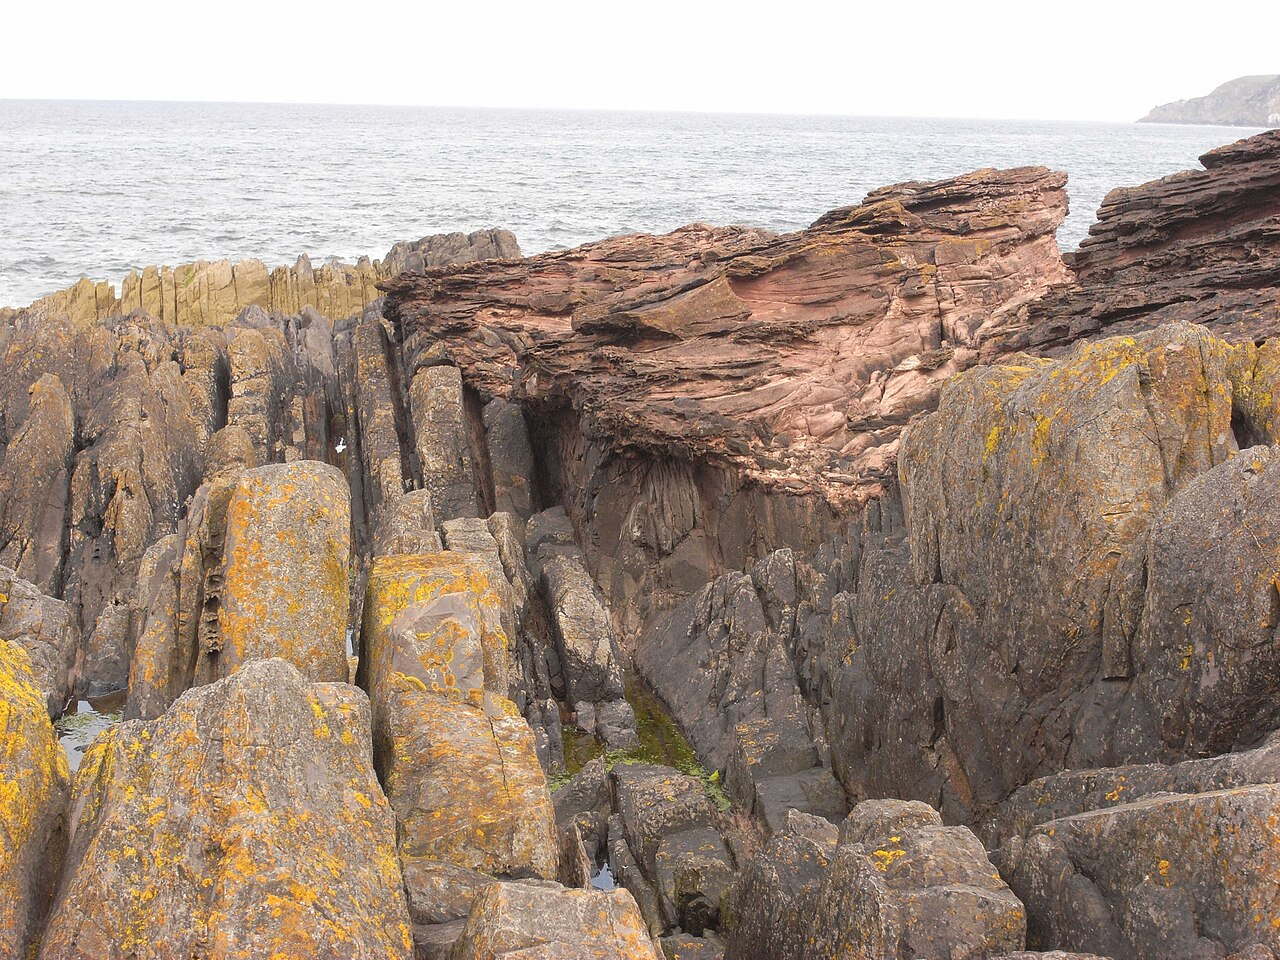
\includegraphics[width=.9\linewidth]{./Figs/Hutton_unconformity_siccar_point.jpg}
    \caption{Siccar Point}
    \label{fig:siccar_point__}
\end{figure}

A \textbf{discordância angular} ocorre quando estratos mais antigos foram inclinados, dobrados ou deformados e, após um intervalo de tempo acompanhado de erosão, passam a ser recobertos por camadas mais jovens depositadas em outra orientação. Nesse caso, o lapso temporal está associado não apenas à ausência de sedimentação contínua, mas também à atuação de processos tectônicos e erosivos entre os dois conjuntos de rochas.

\begin{figure}[H]
    \centering
    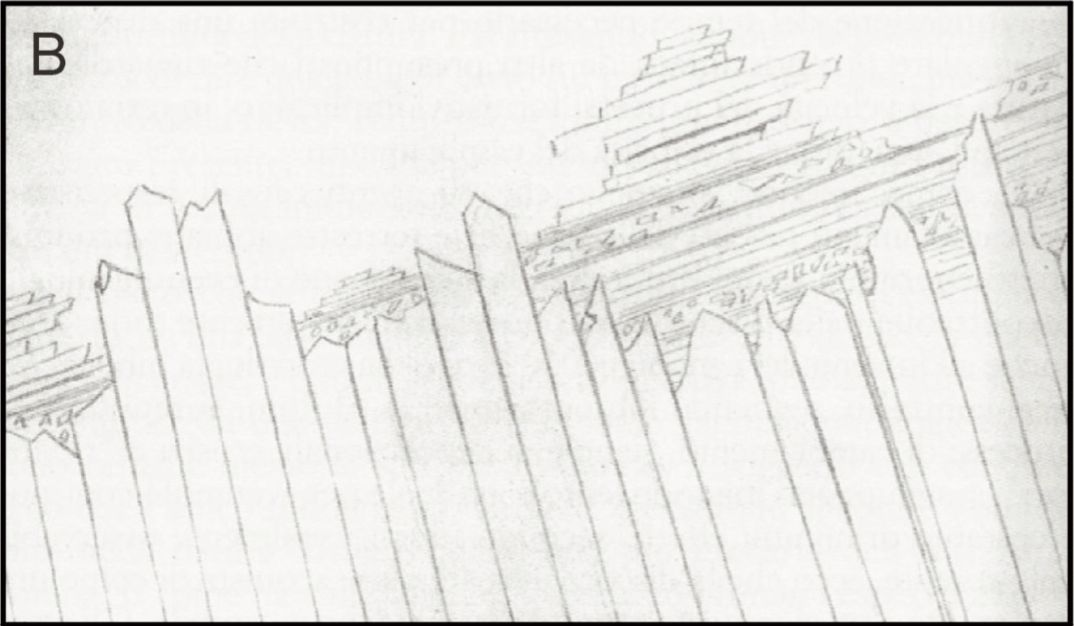
\includegraphics[width=.9\linewidth]{./Figs/Huttons_Unconformity_at_Sicar_Point_by_James_Hall_(1788).jpg}
    \caption{Siccar Point}
    \label{fig:siccar_point}
\end{figure}

A \textbf{desconformidade} ocorre entre camadas sedimentares aproximadamente paralelas, separadas por uma superfície erosiva ou por um hiato de não deposição. Embora a geometria entre os estratos não revele deformação evidente, existe ainda assim um intervalo de tempo ausente no registro, reconhecido pela erosão da superfície ou pela diferença de idade entre as unidades superpostas.

A \textbf{não conformidade} ocorre quando rochas sedimentares repousam diretamente sobre rochas ígneas ou metamórficas mais antigas. Nesse caso, o lapso temporal tende a ser particularmente expressivo, pois envolve a formação das rochas cristalinas em profundidade, sua exumação por soerguimento e erosão, e somente depois o estabelecimento de uma nova fase de sedimentação. Por isso, a não conformidade evidencia de forma especialmente clara a amplitude do tempo geológico envolvido na construção de uma paisagem e de seu registro rochoso.

\begin{figure}[H]
    \centering
    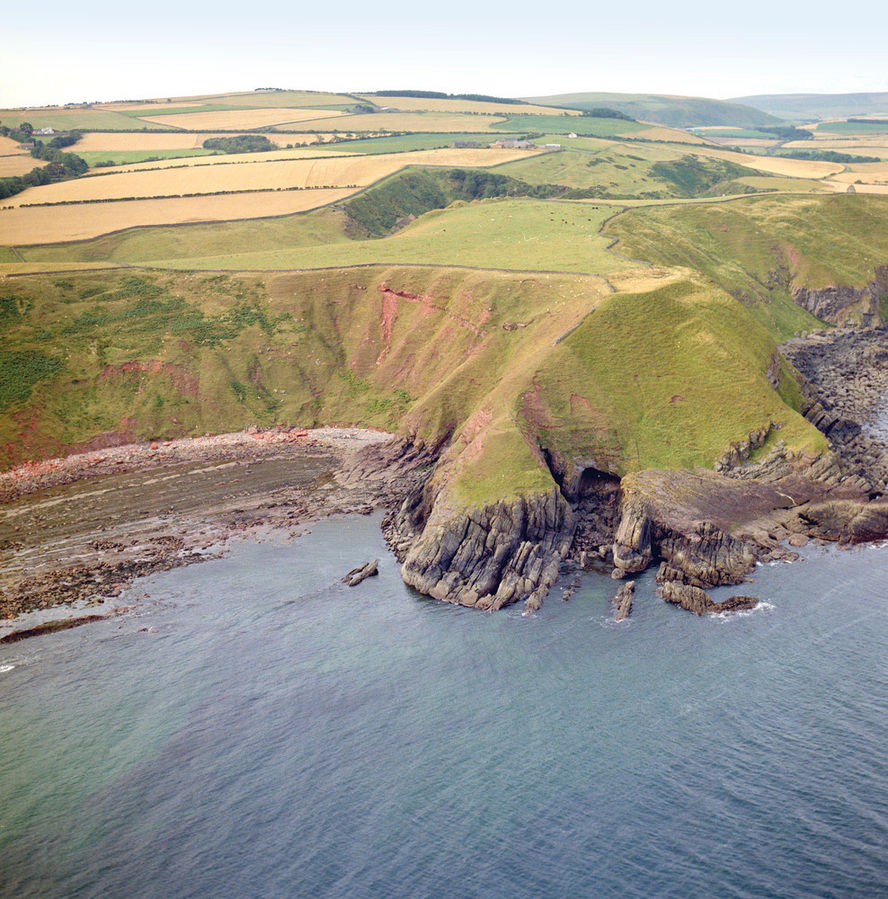
\includegraphics[width=0.9\linewidth]{Figs/afloramento.png}
    \caption{Discordância angular em Siccar Point, Escócia, local clássico associado a James Hutton, onde estratos mais antigos deformados e erodidos são recobertos por camadas sedimentares mais jovens. A feição ilustra a noção de hiato estratigráfico e sua relação com o tempo geológico profundo.}
    \label{fig:aflor}
\end{figure}


Assim, as discordâncias são fundamentais para a interpretação geológica, pois mostram que a história da Terra não é registrada apenas pelos estratos preservados, mas também pelos intervalos de tempo ausentes entre eles. Nesse sentido, a leitura proposta por Hutton foi decisiva ao demonstrar que uma superfície de discordância pode condensar uma longa sucessão de processos geológicos e, portanto, revelar a profundidade do tempo envolvido na evolução da crosta terrestre.
